\documentclass[Cal1Spr16Lectures.tex]{subfiles}

\begin{document}

\section[Week 2]{Week 2: 25-29 January}

% % %
\subsection[2.4 Infinite Limits]{\S 2.4 Infinite Limits}
% % %

% % %
\begin{frame}{\S 2.4 Infinite Limits}
We have examined a number of laws and methods to evaluate limits.  
\begin{que}
Consider the following limit: 
\[
\lim_{x\to 0}\frac{1}{x}
\]
How would you evaluate this limit?
\end{que}
\end{frame}

% % %
\begin{frame}{}\footnotesize
In the next two sections, we examine limit scenarios involving infinity.  The two situations are:
\begin{itemize}
\item {\bf Infinite limits:}  as $x$ (i.e., the independent variable) approaches a finite number, $y$ (i.e., the dependent variable) becomes arbitrarily large or small

\vspace{0.5pc}
\hspace{50pt}looks like: $\displaystyle\lim_{x\to\text{number}}f(x)=\pm\infty$
\item {\bf Limits at infinity:} as $x$ approaches an arbitrarily large or small number, $y$ approaches a finite number

\vspace{0.5pc}
\hspace{50pt}looks like: $\displaystyle\lim_{x\to\pm\infty}f(x)=\text{number}$
\end{itemize}
\end{frame}

% % %
\subsubsection{Definition of Infinite Limits}
\begin{frame}{\small Definition of Infinite Limits}
\begin{dfn}[positively infinite limit] Suppose $f$ is defined for all $x$ near $a$.  If $f(x)$ grows arbitrarily large for all $x$ sufficiently close (but not equal) to $a$, we write
\[\lim_{x \to a} f(x) = \infty\]
and say {\bf the limit of $f(x)$ as $x$ approaches $a$ is infinity}. \end{dfn}
\end{frame}

% % %
\begin{frame}
\begin{center}
\noindent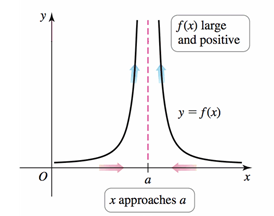
\includegraphics[scale=1]{pictures/Fig2_24a}
\end{center}
\end{frame}

% % %
\begin{frame}
\begin{dfn}[negatively infinite limit] Suppose $f$ is defined for all $x$ near $a$.  If $f(x)$ is negative and grows arbitrarily large in magnitude for all $x$ sufficiently close (but not equal) to $a$, we write
\[\lim_{x \to a} f(x) = -\infty\]
and say {\bf the limit of $f(x)$ as $x$ approaches $a$ is negative infinity}. \end{dfn}
\end{frame}

% % %
\begin{frame}
\begin{center}
\noindent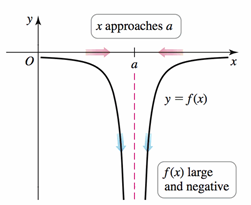
\includegraphics[scale=1]{pictures/Fig2_24b} 
\end{center}
\end{frame}

% % %
\begin{frame}\footnotesize
The definitions work for one-sided limits, too.  

\vspace{1.5pc}
\begin{exe} Using a graph and a table of values, given $f(x)=\displaystyle\frac{1}{x^2-x}$, determine:
\begin{itemize}
\item[(a)\;] $\displaystyle\lim_{x \to 0^+} f(x)$
\item[(b)\;] $\displaystyle\lim_{x \to 0^-} f(x)$
\item[(c)\;] $\displaystyle\lim_{x \to 1^+} f(x)$
\item[(d)\;] $\displaystyle\lim_{x \to 1^-} f(x)$ 
\end{itemize}
\end{exe}
\end{frame}

% % %
\subsubsection{Definition of a Vertical Asymptote}
\begin{frame}{\small Definition of Vertical Asymptote}
\begin{dfn} Suppose a function $f$ satisfies at least one of the following: 

\begin{itemize}
\item $\displaystyle\lim_{x \to a} f(x) = \pm\infty$,
\item $\displaystyle\lim_{x \to a^+} f(x) = \pm\infty$
\item $\displaystyle\lim_{x \to a^-} f(x) = \pm\infty$
\end{itemize}

Then the line $x=a$ is called a {\bf vertical asymptote} of $f$. \end{dfn}
\end{frame}

% % %
\begin{frame}
\begin{exe} Given $f(x)=\frac{3x-4}{x+1}$, determine, analytically (\alert{meaning using ``number sense" and without a table or a graph}), 

\begin{itemize}
\item[(a)\;] $\displaystyle\lim_{x \to -1^+} f(x)$ 
\item[(b)\;] $\displaystyle\lim_{x \to -1^-} f(x)$
\end{itemize}
\end{exe}
\end{frame}

% % %
\subsubsection{Summary Statements}
% % %
\begin{frame}{\small Summary Statements}
Here is a common way you can summarize your solutions involving limits:

\vspace{1pc}
``Since the numerator approaches \alert{(\#)} and the denominator approaches $0$, and is \alert{(positive/negative)}, and since \alert{(analyze signs here)}, \alert{(insert limit problem)}=\alert{($+\infty\,/-\infty$)}."
\end{frame}

% % %
\begin{frame}
Remember to check for factoring -- 

%\vspace{1.5pc}
\begin{exe} \begin{itemize}
\item[(a)] What is/are the vertical asymptotes of 
\[f(x)=\frac{3x^2-48}{x+4} ?\]
\item[(b)] What is $\displaystyle\lim_{x \to -4} f(x)$?  Does that correspond to your earlier answer?
\end{itemize}
\end{exe}
\end{frame}

% % %
\subsubsection{Book Problems}
\begin{frame}
\begin{block}{2.4 Book Problems} 7-10, 15, 17-23, 31-34, 44-45 \end{block}
\end{frame}

% % % 
\subsection[2.5 Limits at Infinity]{\S 2.5 Limits at Infinity}
% % %

% % %
\begin{frame}{\S 2.5 Limits at Infinity}\footnotesize
Limits at infinity determine what is called the {\bf end behavior} of a function.
\begin{exe}
\begin{itemize}
\item[(a) ]Evaluate the following functions at the points $x=\pm100,\pm1000,\pm10000$;
\[f(x)=\frac{4x^2+3x-2}{x^2+2}\qquad g(x)=-2+\frac{\cos{x}}{\sqrt[3]{x}}
\]
\item[(b) ] What is your conjecture about $\lim_{x\to\infty}f(x)$?  $\lim_{x\to-\infty}f(x)$?  $\lim_{x\to-\infty}g(x)$?  $\lim_{x\to\infty}g(x)$?
\end{itemize}
\end{exe}
\end{frame}

% % %
\subsubsection{Horiztonal Asymptotes}
\begin{frame}{\small Horizontal Asymptotes}\footnotesize
\begin{dfn} If $f(x)$ becomes arbitrarily close to a finite number $L$ for all sufficiently large and positive $x$, then we write 
\[\lim_{x \to \infty}f(x)=L.\]
The line $y=L$ is a {\bf horizontal asymptote} of $f$. \end{dfn}  
The limit at negative infinity, $\displaystyle\lim_{x \to -\infty}f(x)=M$, is defined analogously and in this case, the horizontal asymptote is $y=M$.
\end{frame}

% % %
\subsubsection{Infinite Limits at Infinity}
\begin{frame}{\small Infinite Limits at Infinity}\footnotesize
\begin{que} Is it possible for a limit to be both an infinite limit and a limit at infinity? (Yes.) \end{que}

\vspace{0.5pc}
If $f(x)$ becomes arbitrarily large as $x$ becomes arbitrarily large, then we write 
\[\displaystyle\lim_{x \to \infty}f(x)=\infty.\]  

\vspace{0.5pc}
(The limits 
$\displaystyle\lim_{x \to \infty}f(x)=-\infty$, $\displaystyle\lim_{x \to -\infty}f(x)=\infty$, and $\displaystyle\lim_{x \to -\infty} f(x)=-\infty$ are defined similarly.)
\end{frame}

% % %
\begin{frame}{}{}%{\small Infinite Limits at Infinity, cont.}{}
{\bf Powers and Polynomials:}  Let $n$ be a positive integer and let $p(x)$ be a polynomial.

\vspace{1pc}
\begin{itemize}
\item $n=$ even number: $\displaystyle\lim_{x\to\pm\infty}x^n=\infty$ 

\vspace{1pc}
\item $n=$ odd number: $\displaystyle\lim_{x \to \infty} x^n = \infty$ and $\displaystyle\lim_{x \to -\infty} x^n = -\infty$
\end{itemize}
\end{frame}

% % %
\begin{frame}\footnotesize
\begin{itemize}
\item (again, assuming $n$ is positive)
\[\lim_{x\to\pm\infty}\frac{1}{x^n}=\lim_{x\to\pm\infty}x^{-n}=0\]

%\vspace{0.5pc}
\item For a polynomial, only look at the term with the highest exponent:
\[\lim_{x\to\pm\infty}p(x)=\lim_{x\to\pm\infty}\text{(constant)}\cdot x^n\] 
The constant is called the {\bf leading coefficient}, lc$(p)$.  The highest exponent that appears in the polynomial is called the {\bf degree}, $\deg(p)$.
\end{itemize}
\end{frame}

% % %
\begin{frame}\footnotesize
{\bf Rational Functions:}  Suppose $f(x)=\dfrac{p(x)}{q(x)}$ is a rational function.

\begin{itemize}
\item If $\deg(p)<\deg(q)$, i.e., \alert{the numerator has the smaller degree}, then 

\vspace{-1pc}
\[\lim_{x\to\pm\infty}f(x)=0\] 

\vspace{-0.5pc}
and $y=0$ is a horizontal asymptote of $f$.

\vspace{0.5pc}
\item If $\deg(p)=\deg(q)$, i.e., \alert{numerator and denominator have the same degree}, then 

\vspace{-1.5pc}
\[\lim_{x\to\pm\infty}f(x)=\dfrac{\text{lc}(p)}{\text{lc}(q)}\] 

\vspace{-0.5pc}
and $y=\textstyle\frac{\text{lc}(p)}{\text{lc}(q)}$ is a horizontal asymptote of $f$.
\end{itemize}
\end{frame}

% % %
\begin{frame}\footnotesize
\begin{itemize}
\item If $\deg(p)>\deg(q)$, \alert{(numerator has the bigger degree)} then 
\[\lim_{x\to\pm\infty}f(x)=\infty\quad\text{or}\quad -\infty\] 
and $f$ has no horizontal asymptote.

\vspace{0.5pc}
\item Assuming that $f(x)$ is in \alert{reduced form} ($p$ and $q$ share no common factors), vertical asymptotes occur at the zeroes of $q$.  

\vspace{0.5pc}
(This is why it is a good idea to check for factoring and cancelling first!)
\end{itemize}
\end{frame}

% % %
\begin{frame}%\footnotesize
When evaluating limits at infinity for rational functions, it is not enough to use the previous rule to show the limit analytically.

\vspace{1pc}
To evaluate these limits, we divide both numerator and denominator by $x^n$, where $n$ is the degree of the polynomial in the denominator.

\end{frame}

% % %
\begin{frame}%\footnotesize
\begin{exe} Determine the \alert{end behavior} of the following functions (in other words, compute both limits, as $x\to\pm\infty$, for each of the functions):
\begin{itemize}
\item[1.\;] $f(x)=\dfrac{x+1}{2x^2-3}$
\item[2.\;] $g(x)=\dfrac{4x^3-3x}{2x^3+5x^2+x+2}$
\item[3.\;] $h(x)=\dfrac{6x^4-1}{4x^3+3x^2+2x+1}$
\end{itemize}
\end{exe}
\end{frame}

% % %
\subsubsection{Algebraic and Transcendental Functions}
\begin{frame}{\small Algebraic and Transcendental Functions}
\begin{ex} Determine the end behavior of the following functions.
\begin{itemize}
\item[1.] $f(x) = \dfrac{4x^3}{2x^3+\sqrt{9x^6+15x^4}}$ (radical signs appear)

\vspace{1pc}
\item[2.] $g(x)=\cos x$ (trig)

\vspace{1pc}
\item[3.] $h(x)=e^x$ (exponential)
\end{itemize}
\end{ex}
\end{frame}

% % %
\begin{frame}
\begin{exe}
What are the vertical and horizontal asymptotes of $f(x)=\frac{x^2}{2x+1}$?
\end{exe}
\end{frame}

% % %
\subsubsection{Book Problems}
\begin{frame}
\begin{block}{2.5 Book Problems} 9-14, 15-33 (odds), 41-49 (odds), 53-59 (odds), 67  \end{block} 
\end{frame}

\end{document}